\begin{center}
\Huge
Faktorisering af polynomier	
\end{center}
\section*{Faktorisering}
\stepcounter{section}

For ethvert andengradspolynomium $p$ er det muligt at faktorisere det i forhold til polynomiets rødder, hvis de eksisterer. Mere præcist har vi følgende sætning.
\begin{setn}[Faktorisering]
	Lad $p$ være givet ved
	\begin{align*}
		p(x) = ax^2 + bx + c.
	\end{align*}
	Hvis $x_1$ og $x_2$ er rødderne for $p$, så vil $p$ kunne faktoriseres som
	\begin{align*}
		p(x) = a(x-x_1)(x-x_2).
	\end{align*}
	I det specielle tilfælde, at diskriminanten er $0$, så har vi, at 
	\begin{align*}
		p(x) = a(x-x_1)^2.
	\end{align*}
\end{setn}
I tilfældet at diskriminanten er $0$, kalder vi $x_1$ for en \textit{dobbeltrod} eller en \textit{rod med multiplicitet 2}. Det er ikke svært at bevise sætningen, men det kræver lidt regneri. Lad os i stedet betragte et eksempel.
\begin{exa}
	Vi betragter polynomiet $p$ givet ved
	\begin{align}\label{eq:1}
		p(x) = 2x^2 + 6x - 20.
	\end{align}
	Dette har rødderne $x_1 = 2$ og $x_2 = -5$. Vi aflæser, at $a = 2$. Vi bruger sætningen og kan derfor 
	faktorisere polynomiet til
	\begin{align*}
		p(x) = 2(x-2)(x+5).
	\end{align*}
	Hæver vi disse parenteser, så får vi netop udtrykket \eqref{eq:1}.
\end{exa}

\subsection*{Opgave 1}
Et andengradspolynomium $p$ er givet ved
\begin{align*}
	p(x) = 4x^2 + 4x - 8
\end{align*}
og har rødderne $x_1 = 1$ og $x_2 = -2$.
\begin{enumerate}[label=\roman*)]
	\item Faktorisér udtrykket for $p$. 
	\item Hæv parenteserne og se, om faktoriseringen er korrekt. 
\end{enumerate}

\subsection*{Opgave 2}
Et andengradspolynomium $p$ har rødderne $3$ og $-6$ samt $a = -2$.
\begin{enumerate}[label=\roman*)]
	\item Opskriv faktoriseringen for $p$. 
	\item Bestem $b$- og $c$-værdien for $p$. 
\end{enumerate}

\subsection*{Opgave 3}
Et andengradspolynomium $p$ har dobbeltroden $x_1 = 3$ og går gennem punktet $(5,12)$.
\begin{enumerate}[label=\roman*)]
	\item Bestem $a$-værdien for $p$.
	\item Opskriv faktoriseringen for $p$.
	\item Bestem $b$- og $c$-værdien for $p$. 
\end{enumerate}

\subsection*{Opgave 4}
Et andengradspolynomium $p$ er givet ved
\begin{align*}
	p(x) = x^2 + 5x + 6.
\end{align*}
\begin{enumerate}[label=\roman*)]
	\item Bestem rødderne for $p$. 
	\item Opskriv en faktorisering for $p$.
	\item Hæv parenteserne og se, om faktoriseringen er korrekt. 
\end{enumerate}

\subsection*{Opgave 5}
\begin{enumerate}[label=\roman*)]
	\item Aflæs rødderne for følgende parabel.
	\item Opskriv en faktorisering for andengradspolynomiet, der tilsvarer parablen. 
	\item Hæv parenteserne og afgør, om $a$-, $b$- og $c$-værdien tilsvarer parablens udseende. 

\begin{center}
	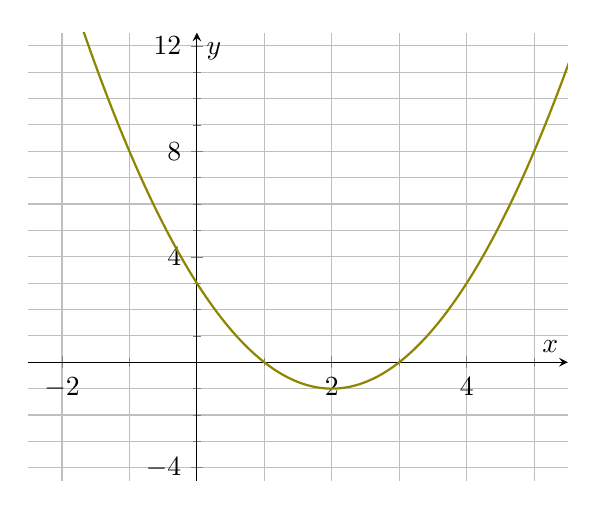
\begin{tikzpicture}
	\begin{axis}[
	axis lines = center,
	xmin = -2.5, xmax = 5.5,
	ymin = -4.5, ymax = 12.5,
	grid = both, 
	xlabel = $x$, ylabel = $y$, 
	xtick = {-4,-2,...,4,6},
	ytick = {-12,-8,...,8,12},
	minor x tick num = 1,
	minor y tick num = 3,
	]
		\addplot[color = olive, thick, domain = -5:6, samples = 200] {2(x-1)*(x-3)};
	\end{axis}
	\end{tikzpicture}
\end{center}


\end{enumerate}

\subsection*{Opgave 6}
Bestem den ukendte koefficient i følgende polynomier, så polynomiet har netop én rod. 
\begin{align*}
	&1) \ p(x) = x^2 + 4x + b &  &2) \ p(x) = ax^2 -6x - 3 \\
	&3) \ p(x) = 2x^2 + bx + 8 &  &4) \ p(x) = ax^2 +10x - 2   \\
\end{align*}


\subsection*{Opgave 7}
Et andengradspolynomium $p$ er givet ved
\begin{align*}
	p(x) = x^2 + bx +c 
\end{align*}
og opfylder, at $p(0) = 5$ og $p(2) = 5$.
\begin{enumerate}[label=\roman*)]
	\item Bestem tallene $b$ og $c$. 
\end{enumerate}

\subsection*{Opgave 8}
Vi vil gerne bevise faktoriseringssætningen. 
\begin{enumerate}[label=\roman*)]
	\item Hæv parentesen i udtrykket $a(x-x_1)(x-x_2)$
	\item Betragt udtrykket. Hvad tilsvarer $b$ og hvad tilsvarer $c$?
	\item Indsæt udtrykket for rødderne fra diskriminantformlen i udtrykkene for $b$ og $c$ og vis, at 
	udtrykket bliver sandt. 
	\item Sæt en sort firkant.
\end{enumerate}
